\chapter{Vertical Light Rays, Tensors, and the Metric}

This lecture begins by filling in a loose end from the equivalence principle and ends by introducing the metric tensor. The path matters. We first ask what happens to a vertical light ray in an accelerating elevator or in a gravitational field, then we sharpen that into a question about frequency shift, then we move to free fall and discover what can and cannot be transformed away. Only after that obstruction is clearly in view do we build the tensor language that will let us describe curved geometry carefully. These notes follow Leonard Susskind's lecture closely; where blackboard frames are kept below, they serve only as documentary support for equations and diagrams, in the spirit of the LazyingArt LLC and Video2Book curation, while the transcript remains the primary guide to the argument.

\section{Vertical Light Rays, Doppler Shift, and the Equivalence Principle}

Susskind begins by returning to a question that was left hanging: not a light ray crossing the elevator, but a light ray traveling vertically. If we shoot an ordinary bullet upward, gravity slows it down; by the time it reaches the ceiling it has less kinetic energy than when it left the floor. That is the familiar Newtonian story.

But light is not an ordinary bullet. Everybody agrees on the speed of light. So when we ask what gravity does to a vertical light ray, the useful question is not whether the speed changes, but what the detector reads when the light arrives. The answer is that the color changes, or in more controlled language, the frequency changes.

Susskind chooses to discuss the downward beam first. Suppose the elevator is momentarily at rest when the beam is emitted from the roof. By the time the beam reaches the floor, the elevator has acquired an upward velocity. The detector on the floor is therefore intercepting the beam while moving relative to the source, and the received light is Doppler shifted. In the accelerating elevator the downward beam is detected slightly blue shifted. By the equivalence principle, the same conclusion applies to a beam fired downward in a gravitational field.

This is not presented as a trick of language. The same effect has been tested near the Earth. Reverse the experiment and the effect reverses with it: a beam sent upward is detected red shifted. Solar spectral lines are correspondingly shifted, and for sufficiently compact objects the effect becomes very large. Susskind emphasizes that the relevant issue is not just size, but compactness; what matters is how hard it is for light to climb out.

\subsection{Question \& Answer}

\paragraph{Question.} Why do the Doppler shifts not simply cancel?

\paragraph{Answer.} They would cancel if the source and the detector differed only by a constant velocity. In that case one shift would be attributed to emission, the opposite one to detection, and the two would undo each other. But here the elevator is accelerating. When the beam is fired, the source is at rest in the chosen frame. By the time the beam arrives, the detector has a different velocity. It is the accelerated motion that makes the later detector velocity differ from the earlier emitter velocity.

Susskind does not write the numerical estimate on the board, but he explicitly assigns it as an exercise. If the height of the elevator is \(h\), then the light travel time is approximately
\begin{equation}
t \approx \frac{h}{c}.
\end{equation}
In that time the detector acquires speed
\begin{equation}
v \approx gt \approx \frac{gh}{c},
\end{equation}
and therefore the fractional frequency shift is of order
\begin{equation}
\frac{\Delta \nu}{\nu} \sim \frac{v}{c} \sim \frac{gh}{c^{2}}.
\end{equation}
For the downward beam the shift is blue; for the upward beam the sign is reversed.

\begin{remark}
The estimate \(\Delta \nu/\nu \sim gh/c^{2}\) is a cautious reconstruction of the exercise Susskind assigns. It is not one of the formulas visibly written on the board in the selected frames.
\end{remark}

The lecture broadens the point immediately after this. Near the Earth the shift is small; for the Sun it is still small but observable; for very compact stars it is larger; near a black hole it becomes enormous. So the opening thought experiment is not just pedagogical. It is already a real physical prediction of the equivalence principle.

\section{Free Fall, Local Cancellation, and Tidal Obstruction}

The next pivot is crucial. An accelerated frame is not something one can fail to notice. If the elevator is being driven upward, one can certainly tell that one is not inertial; one may say either that one is accelerating or that one feels gravity, but one does not mistake the frame for free space. The subtle case is the freely falling elevator.

So we repeat the same experiment in a real gravitational field, but now with the elevator in free fall. Once again Susskind takes a downward beam. There are now two effects to keep track of. The gravitational field by itself would shift the beam one way. But by the time the beam reaches the floor, the floor is itself moving, and that induces an ordinary Doppler shift the other way. The equivalence principle says that in a freely falling elevator these two effects cancel exactly, apart from tidal forces.

We may summarize the local claim as
\begin{equation}
\Delta \nu_{\text{grav}}+\Delta \nu_{\text{Doppler}}=0,
\end{equation}
with the understanding that this is a local statement. Susskind is careful here: if one insists on doing the calculation exactly, one must use special relativity. A purely nonrelativistic treatment leaves a spurious residual at higher order in \(v/c\), whereas the relativistic treatment gives the exact cancellation demanded by the equivalence principle.

\subsection{Question \& Answer}

\paragraph{Question.} Why is there no net shift in a freely falling elevator even though the elevator is accelerating?

\paragraph{Answer.} Because free fall is precisely the situation in which the acceleration of the laboratory compensates for the local effect of gravity. If the cancellation failed, a freely falling laboratory would be distinguishable from an inertial laboratory in empty space, and Einstein's equivalence principle would be wrong. What remains, and what cannot be removed in this way, is only the variation of gravity across the size of the elevator.

That last phrase is the real transition. Gravity near the bottom is not quite the same as gravity near the top. Those leftover effects are the tidal forces. One can remove gravity in a small enough region and for a short enough time, but one cannot remove it globally. There is an obstruction.

Before turning to mathematics, Susskind pauses to reinterpret the accelerated elevator in coordinate language. Meter sticks that are at rest in the elevator trace curved trajectories when viewed from an inertial frame. From outside, one may therefore blame the peculiar phenomena seen by the observer inside the elevator on the use of curved coordinates. In that sense, the ``gravity'' in the uniformly accelerated elevator can be traded for coordinate curvature.

But real gravity due to a planet or star is not exhausted by that story. A freely falling elevator removes most of the effect, not all of it. Tidal forces survive, and so there is an obstruction to removing the gravitational field by a single global coordinate transformation. That obstruction, Susskind now says explicitly, is closely related to the obstruction to removing the curvature of a curved space. That is the bridge into differential geometry.

\section{The Minimal Calculus Toolkit for Curved Coordinates}

Having reached the bridge, the lecture deliberately slows down. We are not yet doing spacetime; for the moment we are speaking only about space. The mathematics, Susskind insists, is not more exotic than multivariable calculus. But we do need two basic rules, and we need them in a notation suited to repeated coordinate changes.

Take a \(d\)-dimensional space with coordinates
\[
x^{1},x^{2},\dots,x^{d}.
\]
A scalar field is simply a function \(\phi(x)\), meaning a single number assigned to each point. Now move an infinitesimal amount. The coordinates change by \(dx^{m}\), and the field changes by \(d\phi\). The first governing formula is the total differential:
\begin{equation}
d\phi=\frac{\partial \phi}{\partial x^{m}}\,dx^{m}.
\end{equation}
This is only the ordinary statement that the change in \(\phi\) is the sum of its directional changes along each coordinate axis.

The next step is the Einstein summation convention. Instead of writing a summation symbol every time, we agree that a repeated index means a sum over that index. Thus
\[
\frac{\partial \phi}{\partial x^{m}}\,dx^{m}
\]
means the sum over \(m=1,\dots,d\). The repeated index is a dummy index: we could have called it \(m\), \(n\), or \(r\); the letter does not matter, provided it does not collide with a free index elsewhere in the same equation.

\paragraph{Coordinate assumptions.} The lecture is explicit that a coordinate system is not arbitrary scribbling. Each point has a unique set of coordinates, and each allowed coordinate map must be one-to-one, continuous, differentiable, and smooth enough for the derivatives we need. The \(d\) in \(x^{1},\dots,x^{d}\) is the dimension of the space, so changing coordinates does not change the number of coordinates. The lecture also pauses briefly to say that all the quantities being multiplied here are ordinary commuting numbers, and that the symbol \(d\) indicates a first-order infinitesimal change, not a finite difference \(\Delta\).

Now introduce a second coordinate system \(y^{n}=y^{n}(x)\). The second governing formula is the chain rule for coordinate change:
\begin{equation}
\frac{\partial \phi}{\partial y^{n}}
=
\frac{\partial \phi}{\partial x^{m}}
\frac{\partial x^{m}}{\partial y^{n}}.
\end{equation}
Susskind spends time unpacking what this means for a fixed \(n\), precisely because it is going to be reused over and over. One first differentiates \(\phi\) with respect to the \(x\)'s, then differentiates the \(x\)'s with respect to the \(y\)'s, and then sums over the repeated index. These two formulas, the total differential and the chain rule, are the small tools from which the tensor machinery will be built.

\section{Scalars, Vectors, and Coordinate Dependence of Components}

Once those rules are in place, the lecture returns to geometry. The key point is that a geometric object is not the same thing as the list of its components. If we overlay one coordinate grid on another, then the same point and the same vector can be described in either system, but the numerical components depend on the coordinates we choose.

\begin{figure}[h]
\centering

\includegraphics[width=0.58\textwidth]{lecture_03_figure_02.png}
\caption{Skew coordinate grid and vector construction. The black and red coordinate families describe the same plane in different ways.}
\end{figure}

\begin{figure}[h]
\centering
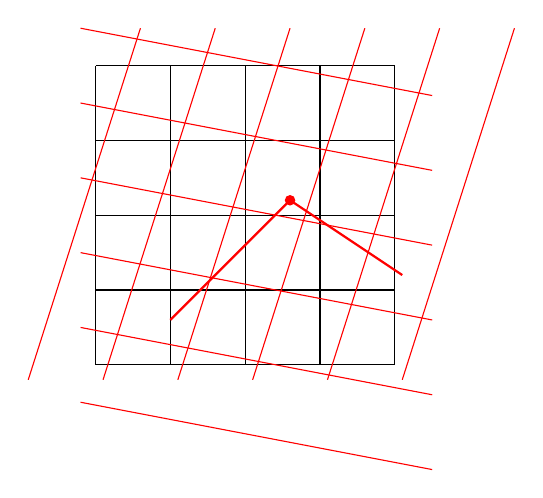
\begin{tikzpicture}[scale=0.95]
\draw[step=1, black, thin] (0,0) grid (4,4);
\foreach \k in {-1,0,1,2,3,4}
  \draw[red, thin] (\k+0.1,-0.2) -- (\k+1.6,4.5);
\foreach \k in {-1,0,1,2,3,4}
  \draw[red, thin] (-0.2,\k+0.5) -- (4.5,\k-0.4);
\fill[red] (2.6,2.2) circle (2pt);
\draw[red, thick] (1.0,0.6) -- (2.6,2.2);
\draw[red, thick] (2.6,2.2) -- (4.1,1.2);
\end{tikzpicture}
\caption{A schematic redraw of the board's point: the geometry stays fixed while the coordinate families change.}
\end{figure}

Susskind begins with the easiest case. A scalar has no directional content. If the \(x\)-coordinates and the \(y\)-coordinates refer to the same point, then the scalar value at that point is the same in both descriptions:
\begin{equation}
\phi(y)=\phi(x).
\end{equation}
This is not yet mysterious. The temperature at a point does not care how we label the point.

\begin{figure}[h]
\centering

\includegraphics[width=0.7\textwidth]{lecture_03_figure_03.png}
\caption{Scalar equality and free vector. The board pairs scalar invariance with the geometric character of the displacement vector.}
\end{figure}

\begin{figure}[h]
\centering
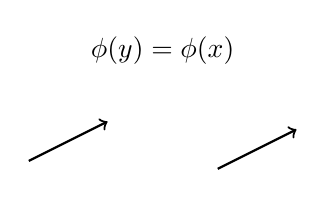
\begin{tikzpicture}[scale=1.0]
\node at (2.5,2.2) {$\phi(y)=\phi(x)$};
\draw[->, thick] (0.8,0.8) -- (1.8,1.3);
\draw[->, thick] (3.2,0.7) -- (4.2,1.2);
\end{tikzpicture}
\caption{A small schematic echo of the board: the same free vector may be drawn in different places without changing the geometric object.}
\end{figure}

We now come to the ``primordial'' vector of the lecture: the infinitesimal displacement. On the board Susskind marks it by an arrow over \(dx\), but the exact chalk styling is not essential. What matters is the idea. The displacement is a geometric object. Its components in the \(x\)-system are \(dx^{m}\), and its components in the \(y\)-system are \(dy^{n}\).

Because each \(y^{n}\) is an ordinary function of the \(x\)'s, we may apply the total-differential formula to \(y^{n}\) itself. That gives
\begin{equation}
dy^{n}=\frac{\partial y^{n}}{\partial x^{m}}\,dx^{m}.
\end{equation}
This is the first nontrivial transformation law in the lecture. The same vector is being described in two coordinate systems, and the components are related by the Jacobian \(\partial y^{n}/\partial x^{m}\).

\begin{definition}
A contravariant vector is a collection of components \(V^{m}\) whose components transform according to
\begin{equation}
V^{n}_{(y)}=\frac{\partial y^{n}}{\partial x^{m}}\,V^{m}_{(x)}.
\end{equation}
The infinitesimal displacement \(dx^{m}\) is the model example.
\end{definition}

The point here is not that a vector is ``made of'' its components. The vector itself is geometric; the components depend on the coordinate frame. That is exactly the lesson carried by the board sketches.

\section{From Vectors to Tensors, and from Contravariant to Covariant}

Once the contravariant vector law is in hand, Susskind does not jump to an axiomatic definition of all tensors at once. He builds the hierarchy. If \(A^{m}\) and \(B^{n}\) are vectors, then the products \(A^{m}B^{n}\) form a rank-two object. Each index transforms the way a vector index transforms, so each index contributes its own Jacobian factor. That is the pattern.

The next important object is not a displacement but a gradient. The collection \(\partial\phi/\partial x^{m}\) has \(d\) components just as \(dx^{m}\) does, but it is geometrically different. It tells us how a scalar field changes along different directions. From the chain rule we read off its transformation law immediately:
\begin{equation}
A^{(y)}_{n}=\frac{\partial x^{m}}{\partial y^{n}}\,A^{(x)}_{m}.
\end{equation}
An object with this transformation law is called a covariant vector. The lecture's model example is the gradient \(A_{m}=\partial\phi/\partial x^{m}\).

This is also where the upstairs and downstairs notation begins to earn its keep. Contravariant indices are written upstairs, covariant indices downstairs. The notation is not yet being presented as deep geometry. At first it is a disciplined bookkeeping system. But it is a very good one: when we sum over indices, we sum an upstairs index against a downstairs index. By inspection we can often see whether an equation is well formed.

A tensor with two lower indices then transforms with one factor of \(\partial x/\partial y\) for each lower index:
\begin{equation}
T^{(y)}_{mn}
=
\frac{\partial x^{r}}{\partial y^{m}}
\frac{\partial x^{s}}{\partial y^{n}}
T^{(x)}_{rs}.
\end{equation}

\begin{figure}[h]
\centering

\includegraphics[width=0.65\textwidth]{lecture_03_figure_04.png}
\caption{Rank-two tensor transformation law. The board shows the covariant two-index rule just before the metric tensor is introduced.}
\end{figure}

The lecture insists on the pattern more than on an abstract definition. A scalar has no indices and does not change. A contravariant vector transforms with \(\partial y/\partial x\). A covariant vector transforms with \(\partial x/\partial y\). A tensor gets one such factor for each of its indices. That is the machinery we need in order to come to the metric.

\section{The Metric Tensor from Pythagoras}

After the break there is a deliberate reset. We now come to the metric tensor, and Susskind starts as simply as possible: with flat space. He is careful to distinguish flat \emph{space} from flat \emph{coordinates}. A flat space can perfectly well be described by curvilinear coordinates. What makes it flat is that there exists at least one coordinate system in which the metric takes the Cartesian form.

Take an infinitesimal displacement \(dx\). Its squared length is \(ds^{2}\). In Cartesian coordinates, Pythagoras gives
\begin{equation}
ds^{2}=(dx^{1})^{2}+(dx^{2})^{2}+\cdots.
\end{equation}
At this point Susskind pauses over notation. The superscript on \(dx^{m}\) labels the coordinate component; it is not an exponent. By contrast, the superscript in \(ds^{2}\) is a genuine square.

One can write the sum schematically as \(dx^{m}dx^{m}\), but that violates the upstairs-downstairs contraction pattern introduced earlier. The cure is to insert the Kronecker delta, defined by
\[
\begin{aligned}
\delta_{mn}&=1 &&\text{when } m=n,\\
\delta_{mn}&=0 &&\text{when } m\neq n.
\end{aligned}
\]
Then the line element takes the cleaner form
\begin{equation}
ds^{2}=\delta_{mn}\,dx^{m}dx^{n}.
\end{equation}
The Kronecker delta picks out the square terms and kills the mixed terms. In Cartesian coordinates it is therefore the metric tensor.

\begin{figure}[h]
\centering

\includegraphics[width=0.62\textwidth]{lecture_03_figure_05.png}
\caption{Metric tensor in Cartesian coordinates. The circled \(\delta_{mn}\) marks the point at which the Cartesian metric is explicitly identified.}
\end{figure}

Now suppose we change coordinates from \(x\) to \(y\). The first step, clearly visible on the board, is
\begin{equation}
dx^{m}=\frac{\partial x^{m}}{\partial y^{r}}\,dy^{r}.
\end{equation}
Substitute this into the line element. The board does this top to bottom, and the layout is pedagogically important: first the coordinate differential, then the substituted line element, then the identification of the new coefficient as the metric.

\begin{figure}[h]
\centering

\includegraphics[width=0.72\textwidth]{lecture_03_figure_06.png}
\caption{Metric tensor under coordinate change. The board circles the coefficient of \(dy^{r}dy^{s}\) and then identifies it as \(g^{(y)}_{rs}\).}
\end{figure}

In clean notation, the argument is
\begin{align}
ds^{2}
&=
g^{(x)}_{mn}\,dx^{m}dx^{n} \\
&=
g^{(x)}_{mn}
\left(\frac{\partial x^{m}}{\partial y^{r}}\,dy^{r}\right)
\left(\frac{\partial x^{n}}{\partial y^{s}}\,dy^{s}\right) \\
&=
\left(
g^{(x)}_{mn}
\frac{\partial x^{m}}{\partial y^{r}}
\frac{\partial x^{n}}{\partial y^{s}}
\right)dy^{r}dy^{s}.
\end{align}
The coefficient in parentheses is precisely the quantity that Susskind circles and names on the board, so we define
\begin{equation}
g^{(y)}_{rs}
=
g^{(x)}_{mn}
\frac{\partial x^{m}}{\partial y^{r}}
\frac{\partial x^{n}}{\partial y^{s}}.
\end{equation}
This is the transformation law of a covariant tensor with two lower indices. The metric is therefore a covariant rank-two tensor.

From this point onward, the metric is the central geometric object. It tells us the distance between neighboring points:
\begin{equation}
ds^{2}=g_{mn}(x)\,dx^{m}dx^{n}.
\end{equation}
To know the metric is to know the local geometry.

\section{Flatness, Curvature, and the Meaning of an Obstruction}

The lecture now cashes out the word obstruction in geometrical language. Suppose we are given a general metric \(g_{mn}(x)\). When does it describe flat space, and when does it describe curved space? Susskind's answer is not a local curvature formula; it is a coordinate question.

\begin{definition}
A space is flat if there exists some coordinate system in which the metric becomes
\[
g_{mn}=\delta_{mn}.
\]
If no coordinate transformation can bring the metric to that form, the space is curved.
\end{definition}

That definition preserves exactly the rhythm of the lecture. We may choose complicated coordinates on a flat space, and the metric may then look complicated. But if there is no obstruction to straightening them out and recovering the Kronecker-delta form, then the space is still flat. Curvature is the obstruction to doing that globally.

This mirrors the earlier physics. In the elevator example one can trade apparent gravity for coordinate curvature. But in a real gravitational field there are tidal leftovers. Likewise, in geometry a general metric may look complicated either because the coordinates are complicated or because the space is genuinely curved. The question is whether the complication can be removed.

The lecture then sharpens the local-versus-global distinction. A space may be locally flat without being globally flat. Indeed, in an infinitesimal neighborhood of a point, one can always flatten the metric. But that does not mean that one can do so everywhere at once. One can also have regions of a space that are flat and other regions that are not.

The cone is the most pointed example in the lecture, in both senses. A cone can be sliced and opened out so that any patch away from the tip becomes flat on the page. But the tip remains a special point. It is an obstruction to finding a single global coordinate system in which the whole cone looks Euclidean. The example is useful because it shows vividly that curvature may be concentrated at a place where every sufficiently small patch away from that place looks flat.

\section{Polar Coordinates as a Worked Flat Example, Then the Sphere}

Having discussed the criterion abstractly, Susskind turns to a concrete metric that looks nontrivial but still describes flat space. Take the plane and replace Cartesian coordinates by polar coordinates:
\begin{equation}
x=r\cos\theta,
\qquad
y=r\sin\theta.
\end{equation}
Differentiate:
\begin{align}
dx &= \cos\theta\,dr-r\sin\theta\,d\theta, \\
dy &= \sin\theta\,dr+r\cos\theta\,d\theta.
\end{align}
Now substitute these into the flat line element \(ds^{2}=dx^{2}+dy^{2}\):
\begin{align}
ds^{2}
&=
\left(\cos\theta\,dr-r\sin\theta\,d\theta\right)^{2}
+
\left(\sin\theta\,dr+r\cos\theta\,d\theta\right)^{2} \\
&=
\left(\cos^{2}\theta+\sin^{2}\theta\right)dr^{2}
+
r^{2}\left(\sin^{2}\theta+\cos^{2}\theta\right)d\theta^{2}
+
0\cdot dr\,d\theta \\
&=
dr^{2}+r^{2}d\theta^{2}.
\end{align}
\begin{equation}
\begin{aligned}
g_{rr}&=1,\\
g_{r\theta}&=0,\\
g_{\theta\theta}&=r^{2}.
\end{aligned}
\end{equation}

This is exactly the tension Susskind wants us to feel. The metric is not a constant array of zeros and ones. One component depends on position. Nevertheless the space is flat, because we know the coordinate transformation back to Cartesian coordinates. The metric looks complicated, but the complication can be undone.

\subsection{Question \& Answer}

\paragraph{Question.} What does the vanishing off-diagonal term actually tell us?

\paragraph{Answer.} In this case it tells us something about the coordinates, not by itself about the intrinsic geometry. The lines of constant \(r\) are circles, and the lines of constant \(\theta\) are straight rays from the origin. The absence of a cross term says that these two families of coordinate lines are perpendicular. If we chose a more awkward curvilinear coordinate system on the same flat plane, then a mixed term \(g_{r\theta}\,dr\,d\theta\) would generally appear. So \(g_{r\theta}=0\) records an orthogonality property of the chosen coordinates; it is not, by itself, a proof that the space is flat.

This clears the way for the final example. The lecture now turns to the sphere. The transcript becomes badly garbled in the surrounding discussion, so the safest thing is to state only the mathematical content that is solidly indicated. For a unit sphere, in the lecture's late notation, the metric is
\begin{equation}
ds^{2}=d\phi^{2}+\sin^{2}\phi\,d\theta^{2}.
\end{equation}
Here the symbol \(\phi\) is no longer the earlier scalar field; it is now an angular coordinate on the sphere.

The point of the example is straightforward even though the late derivation is not fully recoverable from the transcript: unlike the plane in polar coordinates, the sphere cannot be globally straightened so that its metric becomes the Kronecker delta. No matter which coordinates we choose on the sphere, the obstruction remains. That is curvature.

\begin{remark}
The sphere discussion at the end of the lecture is transcriptually unstable. The metric written above is a cautious standard reconstruction consistent with Susskind's notation and with the surviving mathematical content, but the surrounding derivation should be kept brief.
\end{remark}

\section{Summary}

The lecture begins with a physical question about light in an elevator and ends with the metric tensor, and the two halves belong together. A vertical light ray reveals gravitational red shift and blue shift; free fall reveals the exact local cancellation demanded by the equivalence principle; tidal forces reveal the obstruction that remains when one tries to remove gravity globally. That obstruction is then translated into geometry.

From there the mathematical story unfolds step by step. We review the total differential and the chain rule, adopt the summation convention, distinguish scalars from vectors, introduce contravariant and covariant transformation laws, and learn to read the upstairs-downstairs pattern. After the break the metric tensor appears as the coefficient of the line element, and its transformation law shows that it is a covariant tensor of rank \(2\).

The final payoff is geometrical. A space is flat when some coordinate system restores the metric to the Kronecker-delta form. If no such coordinate system exists globally, there is curvature. Polar coordinates show that a complicated metric need not mean a curved space. The sphere shows the opposite lesson: sometimes the obstruction is real.
